% Irodov, Arihant PDF pp. 16--17; original printed pp. 7--8.
% Problems 41--50. Source inconsistencies are recorded where relevant.

\exproblem{41}{7}
质点在平面内运动，其切向加速度恒为 $a_\tau=a>0$，
法向加速度为 $a_n=bt^4$，$b>0$；初始时刻静止。
求曲率半径 $R$ 与合加速度大小 $A$ 关于已走路程 $s$ 的表达式。
\exsolution
由初速为零及切向加速度恒定，
\[
 v(t)=at,\qquad s(t)=\frac12at^2.
\]
曲率半径满足 $a_n=v^2/R$，故 $t>0$ 时
\[
 R=\frac{a^2t^2}{bt^4}=\frac{a^2}{bt^2}
 =\boxed{\frac{a^3}{2bs}}.
\]
把 $t^2=2s/a$ 代入法向分量，有
$a_n=bt^4=4bs^2/a^2$。
所以
\[
 \boxed{A(s)=\sqrt{a^2+\frac{16b^2s^4}{a^4}}
 =a\sqrt{1+\left(\frac{4bs^2}{a^3}\right)^2}.}
\]
\excheck 当 $s\to0^+$，$R\to\infty$、
$A\to a$；表示初始瞬间近似直线加速，不意味着轨迹全程为直线。

\exproblem{42}{7}
质点沿一条平面曲线以恒定速率 $v$ 运动。求 $x=0$ 时的法向
加速度大小及曲率半径，其中轨迹分别为：
(a) $y=ax^2$；(b) $x^2/a^2+y^2/b^2=1$（椭圆半轴 $a,b>0$）。
\exsolution
定速运动切向加速度为零，合加速度完全沿主法线，
大小 $A=v^2/R$。
对平面图像 $y(x)$，
\[
 \kappa=\frac{|y''|}{(1+y'^2)^{3/2}},\qquad R=\kappa^{-1}.
\]
(a) $y'=2ax,\ y''=2a$，在 $x=0$ 有 $\kappa=2|a|$，因此
\[
 \boxed{R_a=\frac1{2|a|},\qquad A_a=2|a|v^2.}
\]
(b) 椭圆的 $x=0$ 两点为 $(0,\pm b)$。在顶部附近选正根
$y=b\sqrt{1-x^2/a^2}$，则 $y'(0)=0$、
$y''(0)=-b/a^2$，故
\[
 \boxed{R_b=\frac{a^2}{b},\qquad A_b=\frac{bv^2}{a^2}.}
\]
底部对称点有相同大小。
\excheck 若 $a=0$，(a) 变成直线，取 $R=\infty$、
$A=0$。椭圆两点的加速度均指向曲线的内侧。

\exproblem{43}{7}
质点 $A$ 沿半径 $R=50\,\mathrm{cm}$ 的圆运动；
由圆上一固定点 $O$ 指向质点的位矢 $\bm r=\overrightarrow{OA}$
以恒定角速度 $\omega=0.40\,\mathrm{rad/s}$ 转动（见原书图1.5）。
求质点速率及合加速度大小与方向。
\begin{center}
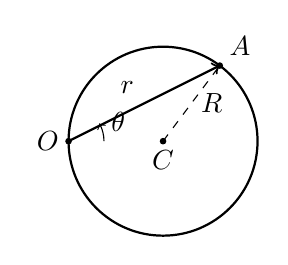
\begin{tikzpicture}[scale=.75]
\coordinate (O) at (0,0);
\coordinate (C) at (1.6,0);
\coordinate (A) at (2.56,1.28);
\draw[thick] (C) circle (1.6);
\draw[->,thick] (O)--(A) node[midway,above left] {$\bm r$};
\draw[dashed] (C)--(A) node[midway,right] {$R$};
\fill (O) circle (1.6pt) node[left] {$O$};
\fill (C) circle (1.6pt) node[below] {$C$};
\fill (A) circle (1.6pt) node[above right] {$A$};
\draw[->] (.6,0) arc (0:30:.6);
\node at (.84,.32) {$\theta$};
\end{tikzpicture}
\end{center}
\exsolution
令 $\theta=\omega t+\theta_0$ 为位矢 $OA$ 与圆心直径 $OC$ 的夹角。
圆心在 $(R,0)$ 时圆的极坐标方程是 $r=2R\cos\theta$。
质点坐标
\[
 x=r\cos\theta=R(1+\cos2\theta),\quad
 y=r\sin\theta=R\sin2\theta.
\]
故质点绕圆心 $C$ 的圆心角速度为 $2\omega$，且恒定。
因此
\[
 \boxed{v=2R\omega=0.40\,\mathrm{m/s}},\qquad
 \boxed{A=\frac{v^2}{R}=4R\omega^2
 =0.32\,\mathrm{m/s^2}}.
\]
\excheck 合加速度始终\emph{沿半径指向圆心 $C$}，并非指向
固定观测点 $O$。图像及解析只在位矢有意义的连续运动段解释。

\exproblem{44}{7}
一轮绕固定轴转动，转角 $\varphi=at^2$，
$a=0.20\,\mathrm{rad/s^2}$。在 $t=2.5\,\mathrm s$ 时，
轮缘点 $A$ 的线速率为 $v=0.65\,\mathrm{m/s}$。
求此刻该点的合加速度大小。
\exsolution
角速度、角加速度分别为
\[
 \omega=2at,\qquad\beta=2a.
\]
轮缘半径由 $v=R\omega$ 得 $R=v/(2at)$。
法向加速度 $a_n=R\omega^2=2at\,v$，
切向加速度 $a_\tau=R\beta=v/t$。
所以
\[
 \boxed{A=\frac vt\sqrt{1+4a^2t^4}
 \simeq0.700\,\mathrm{m/s^2}.}
\]
\excheck 所需半径 $R=0.65\,\mathrm m$，
$a_\tau=0.26\,\mathrm{m/s^2}$、
$a_n=0.65\,\mathrm{m/s^2}$，
勾股合成即 $0.700\,\mathrm{m/s^2}$。

\exproblem{45}{8}
一发炮弹在长 $\ell=2.0\,\mathrm m$ 的炮膛内作匀加速直线运动，
出膛速率 $v=320\,\mathrm{m/s}$。
在炮膛内弹体沿轴向共旋转 $n=2.0$ 圈。求出膛瞬间的自转角速度。
\exsolution
按原书标准求解需采用\emph{等螺距膛线}（弹体每前进相同长度
便转过相同角度）的通常模型。这时累计转角与轴向位移满足
$\varphi=(2\pi n/\ell)x$，故
\[
 \omega_{\rm spin}
 =\frac{\mathrm d\varphi}{\mathrm dt}
 =\frac{2\pi n}{\ell}\frac{\mathrm dx}{\mathrm dt}.
\]
在出膛时
\[
 \boxed{\omega_{\rm spin}=\frac{2\pi n v}{\ell}
 \simeq2.01\times10^3\,\mathrm{rad/s}.}
\]
\excheck 若\emph{只}知道“直线匀加速、共转 $n$ 圈”，
没有等螺距或角加速度规律，实际上不能唯一确定终端角速度。
上述结果以炮膛螺距固定的隐含物理条件为前提。

\exproblem{46}{8}
刚体绕固定轴按 $\varphi=at-bt^2$ 旋转，其中
$a=6.0\,\mathrm{rad/s}$、$b=2.0\,\mathrm{rad/s^2}$。
求：(a) 从 $t=0$ 至第一次停转期间的平均角速度和平均角加速度；
(b) 刚停转时的角加速度。
\exsolution
严格依据\emph{本版所印二次时间规律}，
\[
 \omega=\dot\varphi=a-2bt,\qquad
 \beta=\dot\omega=-2b.
\]
第一次停转时间 $T=a/(2b)=1.5\,\mathrm s$，
累计转角 $\varphi(T)=aT-bT^2=a^2/(4b)$。
因此
\[
 \boxed{\bar\omega=
 \frac{\varphi(T)-\varphi(0)}T=\frac a2
 =3.0\,\mathrm{rad/s},}
\]
\[
 \boxed{\bar\beta=\frac{\omega(T)-\omega(0)}T=-2b
 =-4.0\,\mathrm{rad/s^2},\qquad
 \beta(T)=-4.0\,\mathrm{rad/s^2}.}
\]
\excheck 本版书末给出的 $4\,\mathrm{rad/s}$、
$-6\,\mathrm{rad/s^2}$、$-12\,\mathrm{rad/s^2}$ 等数值
与\emph{印刷题面的二次函数及单位}不符，而与另一个三次时间
模型 $\varphi=at-bt^3$ 的计算相符（此时 $b$ 应为
$\mathrm{rad/s^3}$）。本稿保留原题面并标记此实质性勘误，
不擅自把题面修改为三次方。

\exproblem{47}{8}
刚体从静止起绕固定轴转动，角加速度随时间变化为
$\beta=at$，$a=2.0\times10^{-2}$（依 $\beta=at$ 的量纲，
应取单位 $\mathrm{rad/s^3}$）。
求开始转动后多久，刚体上任意非轴上点的合加速度
与该点的速度成 $\alpha=60^\circ$ 角。
\exsolution
从静止积分，角速度为
$\omega(t)=\int_0^t au\,\mathrm du=at^2/2$。
距轴 $R>0$ 的点的切向、法向加速度为
\[
 a_\tau=R\beta=Rat,\qquad
 a_n=R\omega^2=\frac{Ra^2t^4}{4}.
\]
因速度沿切向，合加速度与速度的夹角满足
\[
 \tan\alpha=\frac{a_n}{a_\tau}=\frac{at^3}{4}.
\]
因此
\[
 \boxed{t=\left(\frac{4\tan\alpha}{a}\right)^{1/3}
 \simeq7.02\,\mathrm s.}
\]
\excheck 结果与距轴距离 $R$ 无关；题面将参数 $a$ 写成
$\mathrm{rad/s^2}$ 属量纲不一致，应注明而非照用。

\exproblem{48}{8}
刚体绕定轴转动，角减速度的大小与 $\sqrt{\omega}$ 成正比，
$\omega\ge0$。初始角速度 $\omega_0>0$。
求从开始到完全停止这段时间的平均角速度。
\exsolution
设比例系数 $k>0$，则
\[
 \dot\omega=-k\sqrt\omega,\quad
 \sqrt{\omega(t)}=\sqrt{\omega_0}-\frac{k}{2}t.
\]
停转时间 $T=2\sqrt{\omega_0}/k$，
因此 $0\le t\le T$ 时
$\omega(t)=\omega_0(1-t/T)^2$。
平均角速度是
\[
 \boxed{\bar\omega=\frac1T\int_0^T\omega(t)\,\mathrm dt
 =\omega_0\int_0^1(1-u)^2\,\mathrm du
 =\frac{\omega_0}{3}.}
\]
\excheck 结果独立于减速比例常数 $k$。
若把条件误抄成 $\beta\propto\omega$，则停转时间无限，
并非本题所述的完整有限停转过程。

\exproblem{49}{8}
刚体角速度与转角的关系为 $\omega=\omega_0-a\varphi$，
$\omega_0,a>0$。初始 $\varphi(0)=0$。
求 $\varphi(t)$ 与 $\omega(t)$。
\exsolution
由 $\omega=\dot\varphi$，
得到一阶线性方程
$\dot\varphi+a\varphi=\omega_0$。
乘以积分因子 $e^{at}$ 并用初值得
\[
 \boxed{\varphi(t)=\frac{\omega_0}{a}(1-e^{-at}),\qquad
 \omega(t)=\omega_0e^{-at}.}
\]
\excheck 角速度逐渐趋零，却只在 $t\to\infty$ 时才严格达到零；
转角趋于有限值 $\omega_0/a$。

\exproblem{50}{8}
刚体自静止起绕固定轴旋转，其角加速度
$\beta=\beta_0\cos\varphi$，$\beta_0>0$，
$\varphi$ 为自初始位置起的转角。
求角速度作为 $\varphi$ 的函数，并画出定性曲线。
\exsolution
利用链式法则
$\beta=\mathrm d\omega/\mathrm dt
=\omega\,\mathrm d\omega/\mathrm d\varphi$，
得
\[
 \omega\,\mathrm d\omega=\beta_0\cos\varphi\,\mathrm d\varphi .
\]
由初始条件 $(\varphi,\omega)=(0,0)$ 积分：
\[
 \frac{\omega^2}{2}=\beta_0\sin\varphi
 \quad\Longrightarrow\quad
 \boxed{\omega=\pm\sqrt{2\beta_0\sin\varphi}},
\qquad \sin\varphi\ge0.
\]
正向初始转动在 $0<\varphi<\pi$ 取正根，
$\varphi=\pi/2$ 时 $\omega_{\max}=\sqrt{2\beta_0}$，
到 $\varphi=\pi$ 停下，随后在相应势能的作用下反转。
\begin{center}
\begin{tikzpicture}[x=1.65cm,y=1.1cm,>=Latex]
 \draw[->] (0,0)--(3.5,0) node[right] {$\varphi$};
 \draw[->] (0,0)--(0,1.8) node[above] {$\omega/\sqrt{2\beta_0}$};
 \draw[very thick,blue!65!black,domain=.1:179.9,samples=100]
 plot ({\x/60},{sqrt(sin(\x))});
 \node[below] at (1.5,0) {$\pi/2$};
 \node[below] at (3,0) {$\pi$};
 \node[left] at (0,1) {$1$};
 \draw[densely dashed] (1.5,0)--(1.5,1);
 \draw[densely dashed] (0,1)--(1.5,1);
\end{tikzpicture}
\end{center}
\excheck 根号中的 $\sin\varphi$ 必须非负；
仅写 $\omega=\sqrt{2\beta_0\sin\varphi}$ 会漏掉反向运动分支。
